\begin{frame}
    \frametitle{Forward Problem}
    \begin{figure}
        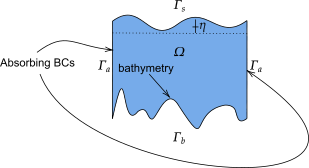
\includegraphics[width=\textwidth]{siam_pp_24/pde-domain-cropped.svg}
        \caption{Illustration of the PDE domain with boundary conditions}
    \end{figure}
    \begin{itemize}
        \item Linearization of the conservation of mass and momentum around hydrostatic pressure in the compressible ocean\footnote{\href{https://link.springer.com/content/pdf/10.1007/s10596-015-9472-0.pdf}{Lotto and Dunham (2015)}}
        \item Assumptions:
        \begin{itemize}
            \item Surface gravity wave height \(\eta \ll\) ocean depth \(\ll\) surface gravity wave length
        \end{itemize}
\end{frame}

\begin{frame}
    \frametitle{Acoustic-Gravity Equations}
    \begin{itemize}
        \item Mixed formulation for Velocity: \(\boldsymbol{u}(x, t)\) and Pressure: \(p(x, t)\)
        \[
        \left\{
        \begin{aligned}
        \rho \frac{\partial \boldsymbol{u}}{\partial t} + \nabla p &= \boldsymbol{0} && \quad \text{in } \Omega \times (0,T) \\
        \frac{1}{K} \frac{\partial p}{\partial t} + \nabla \cdot \boldsymbol{u} &= 0 && \quad \text{in } \Omega \times (0,T)\\
        p = \rho g \eta, \quad \partial_t \eta &= \boldsymbol{u} \cdot \boldsymbol{n} && \quad \text{on } \Gamma_s \times (0,T)\\
        -\partial_t b &= \boldsymbol{u} \cdot \boldsymbol{n}  && \quad \text{on } \Gamma_b \times (0,T)\\
        \boldsymbol{u} \cdot \boldsymbol{n} &= p / \rho c  && \quad \text{on } \Gamma_a \times (0,T)
        \end{aligned}
        \right.
        \]
        \item Boundary conditions:
        \begin{itemize}
            \item ODE type BC on sea surface for Surface Gravity Wave Height: \(\eta(x, t)\)
            \item Seafloor velocity: \(-\partial_t b\) BC on bottom surface (\emph{spatiotemporal parameter field})
            \item 1\textsuperscript{st} order absorbing BC (or PML) on lateral surfaces
        \end{itemize}
        \item \emph{Observations} of pressure \(p\) at seafloor sensors
    \end{itemize}
    \footnotesize{Bulk modulus \(K\), density \(\rho\), \(Z = \rho c\), \(c = \sqrt{K/\rho}\); Homogeneous ICs; Implemented in \href{https://mfem.org/}{MFEM}}
\end{frame}

\begin{frame}
    \frametitle{Weak Formulation}
    \[
    \begin{aligned}
    &\text{Find }
    \boldsymbol{u} \in \mathcal{U},\, p \in \mathcal{V}, \text{such that} \\
    &\int_0^T \! \! \! \int_\Omega
    \left[ \rho\frac{\partial \boldsymbol{u}}{\partial{t}} \cdot \boldsymbol{v} +
    \nabla p \cdot \boldsymbol{v} \right] \text{d} x \text{d} t
    = 0 \, , \quad
    \boldsymbol{v} \in \mathcal{U}, \\
    &\int_0^T \! \! \! \int_\Omega
    \left[ \frac{1}{K}\frac{\partial p}{\partial t} q - \boldsymbol{u} \cdot \nabla{q} \right] \text{d}
    x \text{d} t \,
    +\int_0^T \! \! \! \int_{\Gamma_s}
    \frac{1}{\rho g} \frac{\partial p}{\partial t} q
    \text{d} x \text{d} t
    \\
    +&\int_0^T \! \! \! \int_{\Gamma_a}
    \frac{1}{\rho c} p q
    \text{d} x \text{d} t
    =
    \int_0^T \! \! \! \int_{\Gamma_b}
    \frac{\partial b}{\partial t} q
    \text{d} x \text{d} t
    \, , \quad
    q \in \mathcal{V},
    \end{aligned}
    \]
    \begin{itemize}
        \item Function spaces: \(\mathcal{U} = \boldsymbol{L^2}(\Omega) \times L^2(0,T)\), \(\mathcal{V} = H^1(\Omega) \times L^2(0,T)\) (+ homogeneous ICs)
        \item Surface gravity wave height \(\eta\) recovered from surface BCs
    \end{itemize}
\end{frame}


